\documentclass[UTF8, a4paper]{ctexart}
\usepackage[margin=1in]{geometry} % 页边距调整
\usepackage{ctex}
\usepackage{array, amsmath, amssymb}

\usepackage{booktabs, tabularx, multirow, multicol} % 表格拓展支持
\usepackage{graphicx, subfigure, float} % 图片排版支持

\usepackage{algorithm, algpseudocode} % 伪代码支持
\renewcommand{\algorithmicrequire}{\textbf{Input:}}  
\renewcommand{\algorithmicensure}{\textbf{Output:}} 

\usepackage{tikz, mathpazo} % 基本绘图支持
\usepackage{flowchart} % 流程图支持
\usepackage{pgf-umlcd} % UML类图支持
\usetikzlibrary{arrows, shapes, chains, shapes.geometric}

\usepackage{listings} % 代码块支持
\usepackage{xcolor}
\lstset{
	language		= c++,
	backgroundcolor	= \color{white},
	basicstyle		= \footnotesize\ttfamily,
	keywordstyle	= \color{blue},
	stringstyle		= \color{red!58!blue!82}\ttfamily,
	commentstyle	= \color{darkgray},
	rulesepcolor	= \color{red!20!green!20!blue!20},
	columns			= fullflexible,
	breaklines		= true,
	captionpos		= b,
	tabsize			= 4,
	frame			= single,
	escapeinside	= {\%*}{*)}
}
%%示例
% \begin{lstlisting}[caption={}]
% #include <iostream>
% int main(int argc, char *argv[]) {
% 	std::cout << "Hello World!" << std::endl;
% 	return 0;
% }
% \end{lstlisting}

\usepackage{datetime} %日期
\renewcommand{\today}{\number\year{年}\number\month{月}\number\day{日}}

\begin{document}

\begin{center}
	\zihao{3}《数据结构》实验报告
\end{center}
\zihao{5}

\newcolumntype{Y}{>{\raggedleft\arraybackslash}X}
\noindent\begin{tabularx}{\textwidth}{XcY}
	  {班 级:}\;\underline{DL062123}
	& {姓 名:}\;\underline{项乔栋}
	& {学 号:}\;\underline{2021302468} \\
	  {邮 箱:}\;\underline{13282135976@sina.cn}
	& {日 期:}\;\underline{\today}
	& {编 号:}\;\underline{DS06}
\end{tabularx}
~\\

\noindent\textbf{$\circledcirc$
实验题目:\quad{稀疏矩阵乘法}} \par
\noindent\textbf{$\circledcirc$
实验目的:\quad{实践密集矩阵方法到稀疏矩阵的迁移}} \par
\noindent\textbf{$\circledcirc$
实验内容:\quad{基于十字链表的稀疏矩阵乘法实现}} \par

\subsection*{一、需求分析}
\noindent\fbox{
\begin{tabularx}{\textwidth}{lY}
\bf{Description}
& \parbox[t]{\linewidth}{
	计算两个稀疏矩阵的乘法
} \\

\bf{Input}
& \parbox[t]{\linewidth}{
	首先输入第一个矩阵的行数和列数,再输入该矩阵的三元组形式,以0 0 0结束
	然后输入第二个矩阵的行数和列数,再输入该矩阵的三元组形式,以0 0 0结束
} \\

\bf{Output}
& \parbox[t]{\linewidth}{
	输出相乘后的矩阵三元组
} \\

\bf{Sample Input}
& \fbox{\parbox[t]{\linewidth}{\bf{
	\mbox{3 4 3 2} \\
	\mbox{1 1 1} \\
	\mbox{1 3 1} \\
	\mbox{2 2 2} \\
	\mbox{1 2 1} \\
	\mbox{2 2 3}
}}} \\

\bf{Sample Output}
& \fbox{\parbox[t]{\linewidth}{\bf{
	\mbox{1 1 1} \\
	\mbox{1 2 1} \\
	\mbox{1 3 1} \\
	\mbox{2 3 5}
}}}
\end{tabularx}}

\subsection*{二、概要设计}
十字链表维护了更多的节点信息,天然地具备了有序性。假定实现十字链表的插入操作,那么只需稍微拓展该操作使其支持加和,则原问题就转换为链表遍历与拓展插入的组合。 \par
1.\;基本操作: \par
	CreateFromIO() $\rightarrow$ SparseMatrix \par
	\qquad\textbf{操作结果:}\;从IO流创建稀疏矩阵 \par
	Mul(lhs:SparseMatrix,rhs:SparseMatrix) $\rightarrow$ SparseMatrix \par
	\qquad\textbf{操作结果:}\;获取稀疏矩阵的乘积 \par
	Insert(matrix:SparseMatrix,e:Triple) $\rightarrow$ void \par
	\qquad\textbf{操作结果:}\;向稀疏矩阵插入元素,若元素已存在,则处理元素加和 \par
	Erase(matrix:SparseMatrix,row,col) $\rightarrow$ void \par
	\qquad\textbf{操作结果:}\;删除稀疏矩阵(row,col)处的元素 \par
	Output(matrix:SparseMatrix) $\rightarrow$ void \par
	\qquad\textbf{操作结果:}\;输出稀疏矩阵 \par
2.\;程序模块: \par
1) 主程序 \par
2) IO支持 \par
3) 稀疏矩阵乘法 \par
\begin{figure}[H]
	\begin{minipage}[t]{\linewidth}
		\centering
		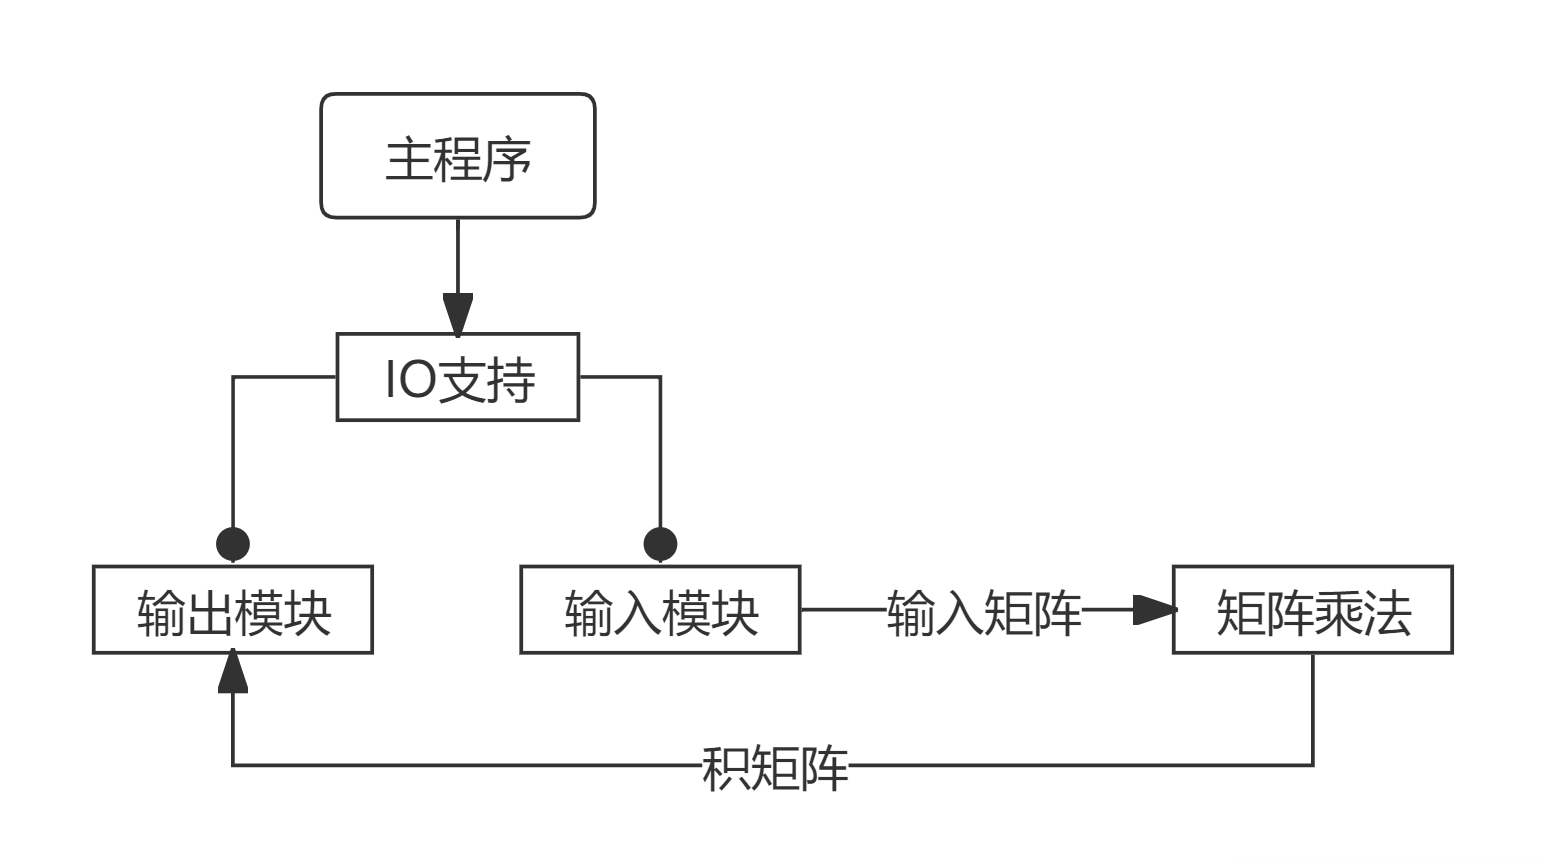
\includegraphics[width=125mm,height=64mm]{./assets/DS06-1}
	\end{minipage}
\end{figure}

\subsection*{三、详细设计}
\begin{algorithm}[H]
\begin{algorithmic}[1]
\caption{Erasure of Orthogonal List}
\Require SparseMatrix: $\mathbf{M}$, Integer: $\mathbf{row},\mathbf{col}$
\Ensure $\mathbf{M}$ with ($\mathbf{row},\mathbf{col}$) erased
\State find e in column $\mathbf{col}$, where e.row = $\mathbf{row}$
\If {e $\neq$ nil}
	\State unlink e from column $\mathbf{col}$
	\State unlink e from row $\mathbf{row}$
	\State release e
\EndIf
\State return $\mathbf{M}$
\end{algorithmic}
\end{algorithm}

\begin{algorithm}[H]
\begin{algorithmic}[1]
\caption{Extended Insertion of Orthogonal List}
\Require SparseMatrix: $\mathbf{M}$, Triple: $\mathbf{E}$
\Ensure $\mathbf{M}$ with $\mathbf{E}$ inserted
\State find last e in row $\mathbf{E}$.row, where e.col < $\mathbf{E}$.col
\If {e.right.col = $\mathbf{E}$.col}
	\State e.value += $\mathbf{E}$.value
	\If {e.value = 0}
		\State erase($\mathbf{M}$, $\mathbf{E}$.row, $\mathbf{E}$.col)
	\EndIf
\Else
	\State let $\mathbf{node}$ $\leftarrow$ $\mathbf{E}$ as orthogonal list node
	\State insert $\mathbf{node}$ after e
	\State fix linkage in column $\mathbf{E}$.col
\EndIf
\State return $\mathbf{M}$
\end{algorithmic}
\end{algorithm}

\begin{algorithm}[H]
\begin{algorithmic}[1]
\caption{Sparse Matrix Multiplication based on Orthogonal List}
\Require SparseMatrix: $\mathbf{A}$,$\mathbf{B}$
\Ensure A$\cdot$B as SparseMatrix
\State let $\mathbf{C}$ $\leftarrow$ SparseMatrix(row=$\mathbf{A}$.row,column=$\mathbf{B}$.column)
\For {p in $\mathbf{A}$.rows}
	\While {p $\neq$ nil}
		\State let q $\leftarrow$ $\mathbf{B}$.rows[p.col]
		\While {q $\neq$ nil}
			\State insert($\mathbf{C}$, p.row, q.col, p.value * q.value)
			\State let q $\leftarrow$ q.right
		\EndWhile
		\State let p $\leftarrow$ p.right
	\EndWhile
\EndFor
\State return $\mathbf{C}$
\end{algorithmic}
\end{algorithm}

\subsection*{四、使用说明、测试分析与结果}
\subsubsection*{1、使用说明}
1) 本程序可以通过任意编译器生成目标文件并在当前平台运行。 \par
2) 进入程序后依照需求的输入样式输入数据,手动输入与流式输入都是被允许的。 \par
3) 请确保输入矩阵的行列标从1开始计数。 \par
\subsubsection*{2、测试结果与分析}
2.1\;\textbf{实际环境} \par
对于所有输入,矩阵元素以行主序输入\par
2.2\;\textbf{边界情况} \par
矩阵积产生零值元素 \par
2.3\;\textbf{测试结果} \par
目标代码通过全部测试,无需纠正
\subsubsection*{3、调试过程问题分析与解决办法}
编码与测试环节皆未产生问题,跳过调试环节
\subsubsection*{4、设计与实现的回顾讨论与分析}
稀疏矩阵的乘法相较于加法与矩阵运算的关联性更强,这在于矩阵乘法的(i,j)位置元素是i行向量与j列向量的点积,而该操作需要对应位置相乘。在稀疏矩阵中,对应位置无元素是很正常的事,故而寻找对应位置的元素是该问题的一个重点。在最简单的矩阵乘法运算中,(i,j)位置的元素是一次计算完成的。然而寻找对应元素在稀疏矩阵中是难的,故而本文中的算法选择分次计算。每当计算出对应位置的一个有效值,就以加和的形式插入到对应位置,那么当算法完成时,(i,j)就自然地成为了行列向量的点积。
\subsubsection*{5、运行界面}
\begin{figure}[H]
	\begin{minipage}[t]{\linewidth}
		\centering
		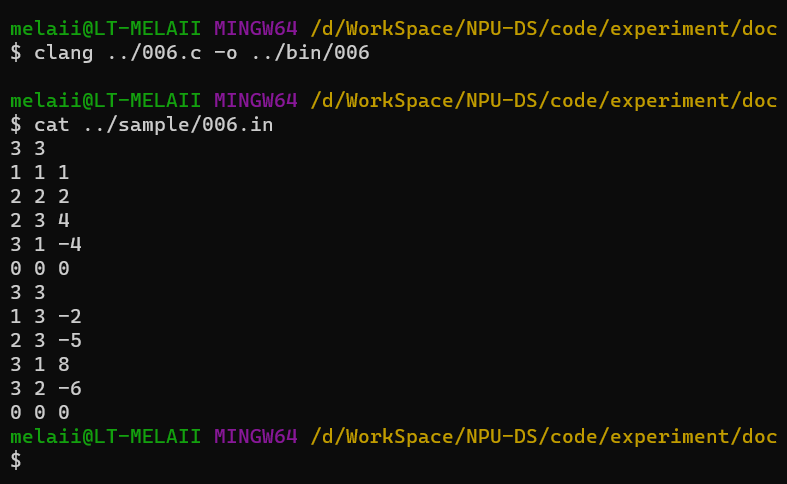
\includegraphics[width=125mm,height=72mm]{./assets/DS06-2}
		\caption{前置环境}
	\end{minipage}
\end{figure}
\begin{figure}[H]
	\begin{minipage}[t]{\linewidth}
		\centering
		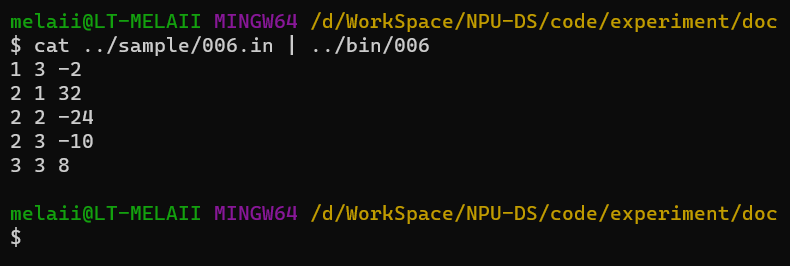
\includegraphics[width=125mm,height=40mm]{./assets/DS06-3}
		\caption{结果输出}
	\end{minipage}
\end{figure}

\subsection*{五、实验总结}
这道题事实上困扰了我很久,题面的三元组给了我误导促使我坚持使用三元表的存储结构,然后三元表过于紧凑的顺序性使得对应元素相乘变得异常困难。诚然暴力遍历可以解决问题,但由于其太过于粗鲁、丑陋被我直接否决,于是最终情况便恶化为迟迟写不出一个能够让我满意的算法。 \par
经过多方面的考虑,我最终打算使用十字链表进行存储,毕竟,题面只是说输入输出时三元组的形式,其实并没有规定要使用该种存储形式。再而,十字链表输出三元组形式也是极其简单的。 \par
考虑十字链表。该结构下,已知前继节点情况下的插入、删除操作都是简单的。且对于完整保存行列头结点的实现,对应行列的元素也能够常数时间得到,这对于矩阵乘法非常有利。 \par

~\\
\zihao{-4}
\textbf{教师评语:}
~\\
\textbf{实验成绩:}

\begin{flushright}
\mbox{指导教师签名:\qquad\qquad} \\
\mbox{批阅日期:\qquad\qquad}
\end{flushright}

\end{document}